\section{Zielsetzung}
\label{sec:Zielsetzung}
Das Ziel des Versuchs ist die Untersuchung der atomaren Gitterstruktur einer Graphitprobe sowie das Analysieren des Höhenprofils einer Goldoberfläche mithilfe eines Rastertunnelmikroskops.

\section{Theorie}
\label{sec:Theorie}
\subsection{Grundlagen der Rastertunnelmikroskopie}
\label{sec:GrundlagenSTM}
Die beschriebenen Grundprinzipien eines Rastertunnelmikroskops basieren auf den Beschreibungen in \cite{Surfaces}.
Ein Rastertunnelmikroskop (STM) ist ein Messgerät, was zur Darstellung der atomaren Struktur vor Oberflächen verwendet wird.
Seine Funktionsweise basiert auf dem quantenmechnanischen Tunneleffekt. 
Dabei durchqueren Elektronen eine im klassischen Sinne unüberwindbare Potentialbarriere. 
Diese Potentialbarriere befindet sich zwischen der metallischen Spitze des STMs und der leitfähigen Probe und besteht in der Regel aus Vakuum. In diesem Versuch ist die Potentialbarriere Luft.
Wird eine Spannung $U$ zwischen der Spitze und der Probe angelegt, können Elektronen durch die Vakuumlücke tunneln, wodurch ein Tunnelstrom entsteht.
Der entstehende Tunnelstrom $I_{\text{T}}$ hängt exponentiell vom Abstand $d$ zwischen der Spitze und der Probe ab. Es gilt die folgende Relation:
\begin{align}
    I_{\text{T}} \propto \frac{U}{d}\exp\left(-K d \sqrt{\varphi}\right)\,, \label{eqn:Tunnelstrom}
\end{align}
wobei $\varphi$ die mittlere Austrittsarbeit und $U$ die angelegte Spannung bezeichnen. 
Für Vakkum gilt dabei $K = \SI{1.025}{\angstrom^{-1} (\eV)^{-1/2}}$.\\

Durch die exponentielle Abhängigkeit des Tunnelstroms vom Abstand $d$ ergibt sich eine hohe Auflösung im Sub-{\AA}ngstrom-Bereich. 
Bereits eine Änderung des Abstands um etwa $\SI{1}{\angstrom}$ kann den Tunnelstrom um eine Größenordnung verändern. Dies macht das STM besonders empfindlich für kleinste topographische Veränderungen an der Probenoberfläche.
Neben der Topographie der Oberfläche wird der Tunnelstrom zusätzlich durch die lokale elektronische Zustandsdichte beeinflusst. 
Daher ist das STM-Bild eine Überlagerung aus topographischer und elektronischer Information.\\

Die Spitze fährt die Oberfläche der Probe rasterförmig ab, wobei der Tunnelstrom im Modus konstanten Stroms aufgezeichnet wird. 
Hierfür wird der Abstand zur Probe durchgänging angepasst, sodass sich ein konstanter Tunnelstrom $I_0$ ergibt. 
Die Steuerung des Spitzenabstands wird über Piezokristalle geregelt, welche eine Bewegung der Spitze in $x$-, $y$- und $z$-Richtung mit subatomarer Präzision ermöglichen. 
% (siehe Abschnitt \ref{sec:Piezokristalle}). 

\subsection{Positionierung und Regelung mit Piezokristallen}
\label{sec:Piezokristalle}
Die präzise Positionierung der STM-Spitze relativ zur Probe wird mithilfe von Piezokristallen kontrolliert.
Diese bestehen meistens aus keramischen Materialien, wie bspw. Blei-Zirkonat-Titanat (PZT), die den piezoelektrischen Effekt nutzen. 
Dabei verformt sich das Material mechanisch, wenn eine elektrische Spannung angelegt wird (inverser piezeolektrischer Effekt). 
Umgekehrt wird beim direkten piezoelektrischen Effekt eine elektrische Spannung erzeugt, wenn das Material mechanisch verformt wird.
Damit dieser Effekt möglich ist, müssen die Piezokristalle bei der Herstellung polarisiert werden. 
Hierzu werden die Kristalle auf etwa \SI{200}{\celsius} erhitzt und gleichzeitig einer Gleichspannung ausgesetzt, wodurch sich die elektrischen Dipole ausrichten \cite{GuidesScanningProbeMicroscope}.\\
\begin{wrapfigure}{r}{0.45\textwidth}
    \centering
    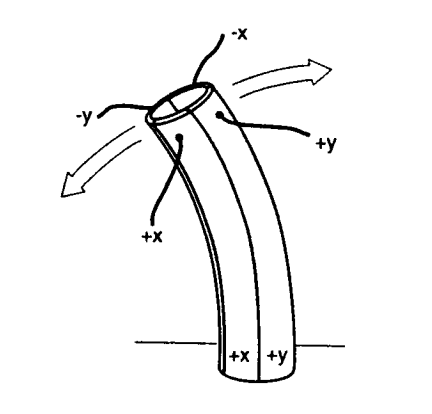
\includegraphics[width=0.43\textwidth]{Bilder/Roehrenscanner.png}
    \caption{Schematischer Aufbau eines Röhrenscanners \cite{GuidesScanningProbeMicroscope}.}
    \label{fig:Roehrenscanner}
\end{wrapfigure}
Im Rastertunnelmokroskop wird die Spitze mit einem sogenannten Röhrenscanner bewegt, wie in \autoref{fig:Roehrenscanner} abgebildet. 
Dieser besteht aus einem zylinderförmigen Piezoelement mit vier Elektroden an der Außenseite, welche Bewegungen in $x$- und $y$-Richtung erzeugen, sowie eine  Elektrode in der Mitte für die Bewegung entlang der $z$-Achse. 
Wenn die äußeren Elektroden unterschiedlich stark angesteuert weden, verformt sich die Röhre und die Spitze bewegt sich in $x$- oder $y$-Richtung.
Wird hingegen auf alle äußeren Elektroden die gleiche Spannung angelegt, dehnt oder staucht sich die Röhre entlang der $z$-Richtung.
Auf diese Weise lassen sich mit hoher Präzision atomare Bewegungen ermöglichen, die für eine rasterförmige Oberflächenabbildung erforderlich sind.
\FloatBarrier

\subsection{Regelung des Spitzenabstands}
\label{sec:PID-Regler}
Im Konstantstrommodus des Rastertunnelmikroskops wird der Abstand zwischen Spitze und Probe kontinuierlich angepasst, um den Tunnelstrom $I_T$ konstant zu halten. 
Dafür sorg eine elektronische Rückkopplungsschleife, in der ein sogenannter PID-Regler (proportional-integral-differential) die nötige Spannung für die Steuerung des $z$-Piezos berechnet.
Der Regler besteht aus drei Komponenten, die zusammen eine präzise und stabile Steuerung des Spitzenabstands ermöglichen.\\

Der proportionale Anteil (P) reagiert direkt auf die momentane Abweichung zwischen Ist- und Sollstrom und sorgt für eine unmittelbare Korrektur.
Der integrale Anteil (I) summiert die vergangenen Abweichungen und gleicht so systematische Fehler über die Zeit aus.
Der differentielle Teil (D) berücksichtigt die Änderungsrate der Abweichung und wirkt stabilisierend, indem er ein Überschwingen der Regelung unterdrückt. Da der Tunnelstrom exponentiell vom Abstand abhängt, reagiert der D-Anteil besonders empfindlich und wird daher typischerweise schwach eingestellt.\\ 

Eine genaue Einstellung dieser Parameter ist entscheidend für die Bildstabilität.
Ist die Regelverstärkung zu niedrig gewählt, reagiert das System nur träge auf Änderungen der Probenoberfläche. Ist sie hingegen zu hoch, kann es zu Instabilitäten oder Überschwingen kommen.
Somit ist der PID-Regler essentiell, um den Spitzenabstand exakt zu steuern \cite{naioManual}.

\subsection{Nichtlineare Effekte und Fehlerquellen bei Piezokristallen}
\label{sec:Fehlerquellen}
Bei der Positionierung der STM-Spitze mithilfe von Piezokristallen treten verschiedene nichtlineare Effekte auf, die sich direkt auf die Bildqualität und Messgenauigkeit auswirken können. Zu den wichtigsten zählen Nichtlinearität, Hysterese, Creep, Cross Coupling sowie Alterung \cite{GuidesScanningProbeMicroscope}.\\

Nichtlinearität beschreibt das Verhalten, dass die Auslenkung der Piezokristalle nicht proportional zur angelegten Spannung verläuft. Dies führt insbesondere bei größeren Scanbereichen zu geometrischen Verzerrungen, da die Bewegung nicht linear skaliert. Der Zusammenhang folgt nicht einem linearen Verlauf, sondern einer S-förmigen Linie.\\

Hysterese tritt auf, wenn der Piezokristall beim Zurückfahren der Spannung einen anderen Verlauf hat, als beim Erhöhren der Spannung.
Dieses Verhalten entsteht, weil sich die elektrischen Dipole im Kristall verzögert zurückbilden. In STM-Bildern führt dies häufig dazu, dass Vorwärts- und Rückwärtsscan nicht identisch sind.\\

Creep bezeichnet die zeitverzögerte Nachverformung des Kristalls nach einer plötzlichen Spannungsänderung. Auch bei konstanter Spannung verändert sich die Position noch über Minuten hinweg leicht. 
Dies kann insbesondere bei langen Scans zu einem langsamen Drift im Bild führen.\\

Cross Coupling bezeichnet die ungewollte Wechselwirkung zwischen verschiedenen Raumrichtungen. 
Da alle Bewegunsrichtungen im Röhrenscannern in einem Bauteil zusammengeführt sind, kann eine Bewegung in $x$- oder $y$-Richtung unbeabsichtigt auch eine Bewegung in $z$-Richtung auslösen. 
Dies erschwert eine präzise Interpretation des Tunnelstroms.\\

Alterung beschreibt die Veränderung der piezoelektrischen Eigenschaften über die Zeit. Wird ein Piezokristall häufig verwendet, richten sich zunehmend mehr Dipole aus, was zu einer stärkeren Dehnung bei kleinen Spannungen führt. Umgekehrt führt eine seltene Nutzung dazu, dass sich die Dipole zufällig ausrichten, wodurch höhere Spannungen erforderlich sind, um dieselbe Auslenkung zu erreichen.\\

Um diese Effekte zu minimieren, gibt es sowohl software- als auch hardwarebasierte Korrekturen.
Bei der Software können Kalibrierungen mit bekannten Referenzstrukturen durchgeführt werden.
So können Algorithmen z.B. geometrische Verzerrungen und Hysterese zu einem gewissen Grad korrigiern.
Bei der Hardware besteht die Möglichkeit, über kapazitive oder optische Sensoren die tatsächliche Position zu messen und aktive gegenzusteuern.
Zusätzlich können Dehnungsmessstreifen zur exakten Auslenkungsmessung beitragen. 
Im hier verwendeten Aufbau des STM werden keine Hardware- und Softwarekorrekturen durchgeführt. 
%Diese  beruhen auf der Kalibrierung des Scansystems mit bekannten Strukturen, um systematische Abweichungen wie Verzerrungen, Skalenfehler oder Hystereseverläufe zu kompensieren. 
%Eine vollständige Korrektur aller Effekte ist auf diesem Weg jedoch nicht möglich, da die Abweichungen von der Probe abhängig sind.

\subsection{Eigenschaften der Proben}
\label{sec:EigenschaftenProben}

\subsubsection{Hochorientierter pyrolytischer Graphit}
\begin{figure}[h]
    \centering
    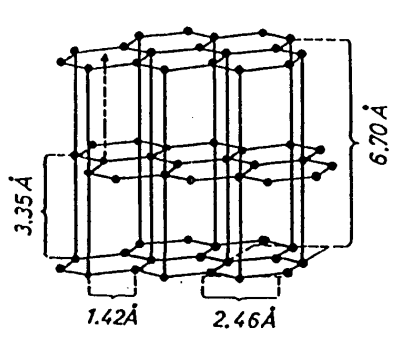
\includegraphics[width=0.5\textwidth]{Bilder/HOPGAufbau.png}
    \caption{Stuktur von HOPG auf atomarer Ebene \cite{ScanningTunnelingMicroscopy}.}
    \label{fig:HOPGAufbau}
\end{figure}
Hochorientierter pyrolytischer Graphit (HOPG) ist eine spezielle Form von Graphit, bei der die Kohlenstoffschichten besonders regelmäßig und parallel zueinander angeordnet sind, wie in \autoref{fig:HOPGAufbau} dargestellt. 
Im Gegensatz zu natürlichem Graphit besitzt HOPG eine deutlich höhere kristallographische Ordnung.
Dies macht das Material besonders gut spaltbar und ist damit ideal geeignet für die Untersuchung im Rastertunnelmikroskop.\\

Die Kristallstruktur von HOPG ist hexagonal mit einer Gitterkonstanten von $a = \SI{2.46}{\angstrom}$. 
Die einzelnen Schichten sind durch Van-der-Waals-Kräfte mit einem Abstand von $c = \SI{3.35}{\angstrom}$ aneinander gebunden. 
Die Schichten sind in einer ABAB-Stapleung angeordnet. Dabei wird innerhalb einer Schicht zwischen A- und B-Sites unterschieden.
A-Sites sind die Kohlenstoffatome, die sich direkt über Atomen der darunterliegenden Schicht befinden.
Dahingegen liegen B-Sites über den Zentren der Sechsecke.
Diese geometrische Anordnung führt dazu, dass die elektronische Kopplung zur unteren Schicht bei A-Sites stärker ausgeprägt ist als bei B-Sites, was die lokale Zustandsdichte an der Oberfläche beeinflusst.\\

In STM-Aufnahmen sind jedoch nicht alle Atome sichtbar. Die A-Sites erzeugen aufgrund ihrer geringeren lokalen Zustandsdiche einen deutlich schwächeren Tunnelstrom. 
Die B-Sites hingegen tragen durch ihre höhere lokalen Zustandsdichte stärker zum gemessenen Tunnelstrom bei. 
Im STM-Bild erscheint dadurch nur jedes zweite Atom, was zu einem Dreiecksmuster führt. Diese Selektion der B-Sites erklärt, warum das sechseckige Gitter optisch nicht vollständig sichtbar ist \cite{ScanningTunnelingMicroscopy}.

\subsubsection{Gold}
Als Vergleichsprobe wird eine (111)-orientierte Oberfläche von Gold untersucht. Im Gegensatz zu HOPG lässt sich unter den im Versuch verwendeten Bedingungen keine atomare Auflösung erzielen. 
Der Grund dafür liegt in der homogeneren Elektronenverteilung auf der Goldoberfläche, wodurch sich keine deutlichen Tunnelunterschiede zwischen benachbarten Atomen ergeben \cite{naioManual}.\\

Stattdessen werden auf der Goldoberfläche größere topographische Strukturen sichtbar. Insbesondere die Stufenkanten sind erkennbar, die entweder durch die natürliche Kristallstruktur des Materials oder als Folge einer mechanischen Vorbehandlung entstehen.
Diese Stufen bilden Höhenunterschiede im Bereich weniger Atomlagen, die mit einem großen Scanbereich zwischen \SI{300}{\nano\meter} und \SI{500}{\nano\meter} abgebildet werden können. Für eine möglichst kontrastreiche Darstellung der Stufenkanten empfiehlt sich eine erhöhte Punktdichte pro Linie, da die Regelschleife bei Gold aufgrund der schwächeren Tunnelstromkontraste langsamer arbeitet \cite{anleitungV42}.
